\documentclass[conference]{IEEEtran}
\usepackage{cite}
\usepackage{amsmath,amssymb,amsfonts}
\usepackage{graphicx}
\usepackage{textcomp}
\usepackage{xcolor}
\usepackage{float}
\usepackage[hidelinks]{hyperref}
\renewcommand{\IEEEkeywordsname}{Keywords}
\begin{document}
\title{AutoGrader: A Rule-Driven Evaluator for C Programs}
\makeatletter
\newcommand{\linebreakand}{\end{@IEEEauthorhalign}\hfill\mbox{}\par\vspace{1em}\mbox{}\hfill\begin{@IEEEauthorhalign}}
\makeatother
\author{
\IEEEauthorblockN{Roshan Jha}
\IEEEauthorblockA{\textit{Computer Science \& Engineering}\\
\textit{IIT Patna}\\
Patna, India\\
roshan\_2611cs23@iitp.ac.in\\
roshanjhazha@gmail.com}
\and
\IEEEauthorblockN{Shivanshu Raj}
\IEEEauthorblockA{\textit{Computer Science \& Engineering}\\
\textit{IIT Patna}\\
Patna, India\\
shivanshu\_2611cs26@iitp.ac.in}
\linebreakand
\IEEEauthorblockN{Mantosh Ravi}
\IEEEauthorblockA{\textit{Computer Science \& Engineering}\\
\textit{IIT Patna}\\
Patna, India\\
mantosh\_2611cs09@iitp.ac.in}
\and
\IEEEauthorblockN{Kanishk Mishra}
\IEEEauthorblockA{\textit{Computer Science \& Engineering}\\
\textit{IIT Patna}\\
Patna, India\\
kanishk\_2611cs20@iitp.ac.in}
}
\maketitle


\begin{abstract}AutoGrader evaluates student C programs using bounded execution, source analysis, runtime diagnostics, and optional local language-model review. A Python coordinator reads external rules, dispatches nine analyzers, and combines their scores into an overall grade. The browser interface provides registration, metric charts, test evidence, and downloadable reports. Six sample submissions evaluated under the assignment preset received grades from 39.3 to 92.0. The baseline scored 82.3 and triggered a signed-overflow diagnostic despite matching every expected output, demonstrating the value of separate correctness and memory-safety checks. This paper presents the implemented architecture, methods, recorded results, and deployment limitations. Model unavailability activates documented heuristics, while timing noise and environment changes constrain strict reproducibility. The prototype supports supervised coursework feedback and motivates further evaluation on broader submission sets.\end{abstract}

\begin{IEEEkeywords}automated grading, C programs, static analysis, sanitizers, rule-based scoring, local language models.\end{IEEEkeywords}

\section{Introduction}

Evaluating C assignments requires checking output, runtime behavior, and code quality. A passing test can conceal undefined behavior, while correct output alone gives little evidence of decomposition or readability. AutoGrader coordinates these checks through an external rubric and reports the evidence behind each score.

The instructor supplies the statement, reference solution, tests, and grading policy. The student submits a C file and receives a weighted result with explanations. Keeping the rubric outside the coordinator makes assessment criteria explicit and supports changes without editing the grading engine.

\newpage

\subsection{Project scope and contributions}

The implemented system supports local Linux execution and Windows operation through Ubuntu in WSL2. Its main contributions are an external nine-metric rubric, coordinated source and execution analysis, concrete counterexamples, and a visual report that relates each deduction to its evidence. The current interface also includes registration, sign-in, and sign-out for addresses ending in @iitp.ac.in.


The term agent refers to an application-level coordinator that selects and executes analysis stages from rules. Language-model calls supplement several stages, while the weighted total is computed in Python. The demonstrated results use the documented fallback path because Ollama was unavailable during evaluation.


\subsection{Requirements from the assignment}

The assignment calls for unattended evaluation, fixed time and memory limits, independently implemented metrics, configurable weights, and feedback containing a failing input with its expected output \cite{ref1}. It also requests suspected-copying flags, sample outputs, and three to four concrete examples of usefulness and limitations. These requirements guide the repository structure and report contents.


The assignment's reproducibility contract is especially demanding. Recording a source hash and a rules hash helps identify an evaluation, but the observed grade also depends on compiler behavior, model availability, the comparison corpus, and runtime measurements. This report distinguishes the implemented controls from the stronger guarantee still requiring further work.


\newpage

\section{System Architecture}

\subsection{User-facing workflow}

The browser opens a sign-in page. A new user registers an institutional email address and then signs in using that address. Inside the grader, the user selects a rules preset, uploads a .c file or chooses an example, and starts grading. Figure 1 summarizes this sequence. The user may revise the source and repeat the evaluation after reading the feedback.


\begin{figure}[H]\centering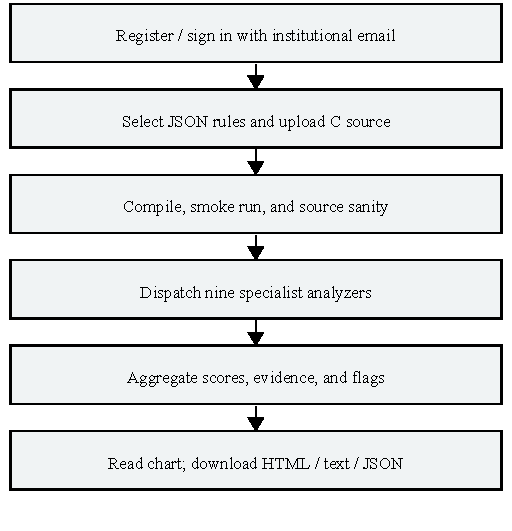
\includegraphics[width=\columnwidth]{workflow.pdf}\caption{User workflow and coordinated evaluation stages. The command-line interface invokes grading directly.}\label{fig:1}\end{figure}

\subsection{Web access and interface}

The FastAPI application in web\_access.py mounts the Gradio interface at /grader. Gradio supplies file input, preset selection, report components, and client/API interactions \cite{ref3}. The access middleware and authentication dependency gate the grader and associated uploads and downloads. The interface displays explicit light- and dark-mode colors for metric bars, text, and evidence panels.


SQLite stores registered email addresses under the Linux user's application-data directory. Random session tokens are held in server memory and placed in HTTP-only cookies. Sessions last eight hours and end on logout or a server restart. The current flow checks registration and the email suffix; mailbox ownership is unverified. Consequently, another person who knows a registered address can sign in with it.


\newpage

\subsection{Coordinator and execution context}

The front\_app.py entry point handles browser and command-line input. The coordinator loads rules through rules\_loader.py, creates a temporary working directory, and constructs a Context containing the source, problem statement, limits, and paths. The context supplies common accessors for known inputs, rule-relative paths, and model configuration.


The first pass compiles with GCC using optimization, common warnings, and C11 mode. It then executes a smoke input and checks for a main function, input and output calls, and a return statement. A compilation failure or smoke timeout produces a partial report. Execution-dependent metrics are skipped, while source-only analyzers continue.


Independent analyzers run in a thread pool capped at three workers. The timing-sensitive complexity stage runs separately to reduce interference from the other analyzers. Each result includes a bounded score, evidence, feedback, suggestions, and optional flags. Exceptions are converted into analyzer-error results so that the evaluation can still produce a report.


\subsection{Module responsibilities}

The sandbox module owns compilation and execution. Source parsing utilities support function extraction and token analysis. The llm\_client module centralizes local model calls and caching. The report\_writer module writes text, JSON, and HTML files, while result\_analysis generates the chart and evidence-based narrative.


The rules directory contains both the assignment preset and the original addition exercise. Each problem directory holds its statement, reference solution, and paired input/output files. The samples directory supplies six programs with different behaviors. Saved assignment outputs reside in sample\_reports/agentic\_ai.


\subsection{Data ownership and lifecycle}

Temporary binaries are removed after grading. Report filenames are derived from the submitted source basename, so later runs with the same basename replace those outputs. Accounts persist separately from report files, while sessions expire in memory. Per-user report isolation and versioned submissions remain deployment work. For the present single-machine demonstration, downloading reports provides an explicit way to retain a particular result.


\newpage

\section{Analysis Methods}

\subsection{Correctness and edge cases}

The correctness analyzer executes each supplied input and compares actual output with the paired expected output. A passing case requires successful termination and an output match. Its score is the fraction of tests passed. Failure evidence records the input, expected output, actual output, and execution status.


The edge-case analyzer resolves named groups such as negatives, zero, and integer overflow. Expected values are obtained by running the instructor's reference solution. Optional model-generated counterexamples are also compared against the reference. Their effect on the grade is controlled by the extra\_cases\_count\_in\_score setting; the default treats them as additional feedback.


\subsection{Compiler and source-level checks}

The syntax analyzer recompiles with the requested warning flags and deducts a configurable amount per warning. It removes -Werror during counting so that warnings remain observable. An actual compilation error yields a zero syntax score. The default warning penalty is 0.1 on the normalized scale.


Structure analysis estimates function complexity and length using the repository's C-source utilities. The assignment limits cyclomatic complexity to eight and function length to forty lines. Cppcheck contributes additional warning, style, performance, and portability findings. Cppcheck is a static C/C++ analysis tool designed to identify suspicious constructs and undefined behavior \cite{ref4}.


Modularity analysis counts defined functions and identifies called helper functions. The assignment requests at least two functions. This tests a particular instructional preference: a short but correct single-function solution can lose modularity points under this rubric.


\subsection{Runtime memory diagnostics}

The memory analyzer recompiles with AddressSanitizer and UndefinedBehaviorSanitizer and runs the known inputs. GCC's instrumentation options provide runtime checking for memory errors and selected undefined operations \cite{ref5}. Distinct issue categories determine deductions, with the first triggering input retained as evidence. The default penalty is 0.3 per distinct issue.


For diagnostics linked to supplied tests, the report includes expected and actual output alongside the sanitizer finding. This matters when a program prints a matching value while executing a signed-overflow operation. A clean sanitizer run establishes coverage only for the executed inputs.


\newpage

\subsection{Empirical complexity}

The complexity estimator runs configured input sizes repeatedly, uses median runtimes, and measures a startup baseline. A log-log growth estimate is classified into a complexity category and compared with the required bound. The assignment uses sizes 1, 10, and 100 and requires O(1). Timings below a configured noise floor can be classified as constant.


For the two-integer input pattern, increasing the configured size changes numeric values rather than the number of input elements. The resulting timing evidence is narrow and cannot establish general algorithmic complexity. Larger tasks need problem-appropriate generators and sizes that produce measurable work.


\subsection{Readability and originality}

Readability uses a rubric prompt sent to a local Ollama chat endpoint \cite{ref6}. Responses supply a score, reasons, and suggestions. With an unavailable model or invalid response, a source heuristic assigns 40\% to comment presence, 40\% to identifier length, and 20\% to short lines. The fallback status appears in the report.


Originality normalizes tokens and compares token four-gram sets with the local corpus using Jaccard similarity. The assignment flags a maximum similarity above the configured 0.85 threshold and assigns zero originality points when flagged. Optional comparisons with model-generated solutions produce advisory LLM-copy flags. Corpus matching covers the reference files supplied locally.


\section{Scoring And Contract}

For metric $i$, let $s_i$ denote a score in $[0,1]$ and $w_i$ its nonnegative configured weight. The final grade is

\begin{equation}G=100\,\frac{\sum_i w_i s_i}{\sum_i w_i}.\label{eq:grade}\end{equation}

The assignment gives correctness weight 0.20 and each of the other eight metrics weight 0.10. Rules with a positive total weight are normalized when needed. Skipped execution metrics retain zero scores and their configured weights in a partial report. Analyzer errors also return zero scores with explicit error evidence.


The assignment preset expects signed 32-bit wrapped output, including -2147483648 for input 2147483647 1. Its reference uses wider arithmetic to implement that output safely. The original exercise instead expects the mathematical sum 2147483648. The selected contract explains several result differences in Section V.


\newpage

\section{Evaluation And Results}

\subsection{Evaluation setting}

The evidence consists of saved JSON reports for six supplied C programs, evaluated using rules/agentic\_ai.json on the local Ubuntu/WSL setup. Reports record GCC 15.2.0 and Cppcheck 2.19.0. The example suite contains ten ordinary tests and named boundary cases. Ollama was unavailable, so readability used the heuristic fallback and AI-specific extra checks were skipped.


This is a small functional demonstration. It provides no estimate of grading accuracy on a representative student population and no throughput benchmark. The displayed values are transcribed from actual report files rather than generated to match the illustrative score in the assignment.


\begin{table}[H]\caption{Saved results under the assignment preset}\label{tab:1}\centering\begin{tabular}{lrr}\hline
Submission & Grade & Report \\\hline
add\_basic.c & 82.3 & Complete \\
add\_buggy.c & 83.7 & Complete \\
add\_clean.c & 92.0 & Complete \\
add\_copy.c & 80.0 & Complete \\
add\_infinite\_loop.c & 39.3 & Partial \\
add\_leak.c & 86.3 & Complete \\\hline\end{tabular}\end{table}

\begin{figure}[H]\centering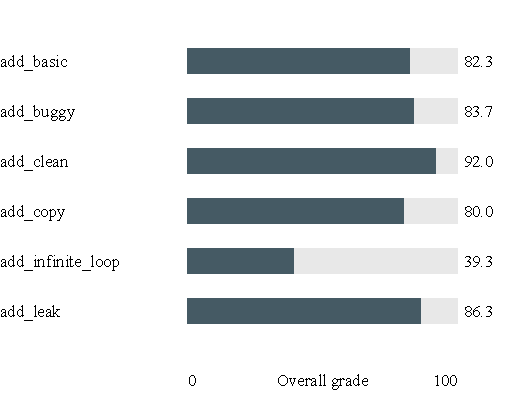
\includegraphics[width=\columnwidth]{results.pdf}\caption{Saved overall grades under the assignment preset. The infinite-loop result is partial and retains zero scores for skipped metrics.}\label{fig:2}\end{figure}

The grade is a rubric aggregate. The buggy program scores above the basic program because stronger modularity and readability can outweigh lost correctness points. Instructors who require correctness to dominate should adjust weights or define an explicit eligibility policy.


\newpage

\subsection{Baseline example analysis}

The assignment's compact addition example and add\_basic share the relevant baseline behavior. The example receives 82.3/100. It passes all ten output tests and all ten configured edge cases but triggers a signed-overflow diagnostic on input 2147483647 1. Table II shows the point contributions.


The largest deduction is seven points for modularity because only main is defined. Memory safety loses three points for a sanitizer issue. Syntax loses one point for ignoring scanf's return value. The readability heuristic contributes 3.33 out of ten. Summing the displayed contributions yields approximately 82.33, which is rounded to 82.3.


\begin{table}[H]\caption{Baseline metric contributions}\label{tab:2}\centering\begin{tabular}{lrr}\hline
Metric & Available & Earned \\\hline
Correctness & 20 & 20.00 \\
Syntax & 10 & 9.00 \\
Structure & 10 & 10.00 \\
Modularity & 10 & 3.00 \\
Logical & 10 & 10.00 \\
Complexity & 10 & 10.00 \\
Memory safety & 10 & 7.00 \\
Readability & 10 & 3.33 \\
Originality & 10 & 10.00 \\\hline\end{tabular}\end{table}

\subsection{Other behaviors and verification}

The clean sample earns 92.0 under the wrapping preset because its mathematical-sum behavior differs on overflow cases. The copy sample loses its originality contribution. The infinite-loop sample is stopped during the smoke run and receives a partial report. The leak sample receives a memory-safety deduction. These distinct outcomes exercise useful branches of the pipeline.


Local verification submitted the assignment example through the Gradio client, checked nine metric rows and overflow evidence, and confirmed three downloadable report files. A temporary account database exercised rejection of an incorrect email suffix, registration, sign-in, authenticated grading, and logout revocation. Browser checks inspected light and dark report colors. These checks establish the exercised flows; broader concurrency and adversarial security testing remain necessary.


\newpage

\section{Installation And Operation}

\subsection{Reproducing the local setup}

The repository README provides the clone URL and installation commands \cite{ref2}. On Ubuntu or Debian, install Git, build-essential, cppcheck, python3-venv, and python3-pip. Clone the repository and run bash run-local.sh. The script creates .venv-linux and installs requirements.txt. The browser opens the application at http://127.0.0.1:7860.


On Windows, install Ubuntu with WSL2 and complete the Linux user setup. Firmware virtualization and the Virtual Machine Platform component must be available. Start-AutoGrader.cmd invokes the Linux launcher. The project uses Linux process and resource controls for C execution, so a native Windows Python installation alone is insufficient.


The optional Ollama model must be installed and reachable from the same environment. The selected rule file specifies the host, model, temperature, and seed. Offline operation retains the non-model analyzers and marks the fallback in the report. This supports demonstrations on machines without a model while making the changed evaluation path visible.


\subsection{Resource controls and trust}

Ordinary execution uses a one-second wall-clock limit and a 64 MB virtual-address-space cap in the assignment preset. Bash resource limits also constrain CPU time and output-file growth. Input and output use temporary files to avoid pipe deadlocks. Process groups allow cleanup after timeouts and after ordinary completion.


Sanitizer builds require a different execution allowance. Their large virtual-memory reservations require disabling the address-space cap, and the analyzer uses a timeout five times the ordinary limit. These conditions are important when interpreting the nominal memory limit in the interface.


The current controls protect against many buggy programs. Submitted code still executes with the Linux user's permissions, and the application has no hardened filesystem or namespace isolation. Public arbitrary-code execution needs a separately isolated worker and security review. Email-only access also permits impersonation of a known registered address. These are explicit boundaries of the local prototype.


\subsection{Report retention}

HTML reports can be read offline and include metric bars and expandable evidence. Text reports support concise review, while JSON retains machine-readable details. Repeated source basenames overwrite the same report paths. Versioned storage and user-owned report access are important extensions for shared operation.


\newpage

\section{Usefulness And Limitations}

\subsection{Four practical uses}

Coursework feedback. In a lab with 300 submissions, repeated compilation and test execution can be automated while instructors review ambiguous cases. A student can reproduce the exact boundary input reported by the grader.


Interview practice. A training group can apply the same editable rubric across candidate solutions and examine differences in correctness, decomposition, and memory behavior. This offers structured feedback for subsequent revision.


Originality triage. An instructor can compare submissions with a local corpus and inspect pairs above the threshold. Prioritizing those pairs can reduce manual search effort while retaining human judgment.


Student self-check. A learner can evaluate a program locally before submission, inspect an overflow or leak finding, and rerun after a change. The chart makes the distribution of points visible across the nine metrics.


\subsection{Four concrete failure modes}

Incomplete test coverage. A program can hardcode the ten expected answers and pass those cases while failing on a new legal input. More varied reference-based inputs and rotating test suites improve coverage, but finite testing still leaves unobserved behaviors.


Misleading timing estimates. Bubble sort on tiny arrays can finish below the noise floor and appear constant-time. Startup cost, operating-system scheduling, and concurrent load also distort growth curves. Use larger problem-specific inputs and retain the raw timing evidence.


Ambiguous similarity. Two students can independently write almost identical short addition programs and exceed the threshold. Conversely, reordered or padded copied code can evade the token comparison. Thresholds need calibration, and flagged cases need manual review.


Unstable readability judgments. Comment count and identifier length can reward superficial changes. A language model can also follow misleading source comments or vary across versions. Fixed prompts, cached responses, and instructor spot-checks reduce some uncertainty.


These limitations affect interpretation of the total. A grade accompanied by evidence is more informative than a single number, particularly when output tests pass while diagnostics reveal undefined behavior. The current reports expose these conflicts rather than requiring the student to infer them from the final score.


\newpage

\section{Discussion And Future Work}

\subsection{Reproducibility and evidence integrity}

The source SHA-256 and canonical rules hash identify two inputs to an evaluation. Local model responses are cached using the model settings and prompts, and requests fix seed and temperature. Expected edge outputs come from the reference solution. These controls help reproduce the demonstrated workflow, but the full evidence state is broader than the current hashes.


Changing a test file or a corpus file without changing its path can affect the grade while leaving the rules hash unchanged. Timing noise, tool upgrades, model availability, and platform-dependent undefined behavior can also change observations. A more complete record would fingerprint the tests, reference source, corpus, prompt files, environment, and scoring configuration together.


The current denominator retains skipped metrics. This penalizes programs that cannot reach execution-dependent checks, but an infrastructure error may also yield a zero contribution. An improved policy should distinguish student failures from unavailable tooling and explicitly define when a result is provisional. Such a policy would require instructor agreement and regression tests before changing existing grades.


\subsection{Prioritized extensions}

First, strengthen isolation with disposable execution workers, filesystem restrictions, per-job resource accounting, and careful cleanup. Second, replace email-only access with verified institutional authentication and add user-owned, versioned report storage. Third, expand the problem library and validate reference solutions independently for each exercise.


Further measurement work should include a larger labeled submission set, repeated runs on multiple machines, tool-version comparisons, and calibration of complexity and similarity thresholds. A controlled model-enabled study could compare readability judgments with instructor ratings. These studies would support quantitative claims beyond the present six-sample demonstration.


\subsection{Evaluation priorities}

A useful next evaluation would separate rubric agreement from runtime reliability. Instructor scores on a larger, independently reviewed submission set would support agreement analysis for each metric. Repeated execution would reveal how frequently grades change with load, tool versions, or unavailable services. The two studies address different sources of uncertainty and should report their conditions separately.


The present evidence supports successful completion of the exercised local workflows. It leaves open the rate of false similarity flags, the quality of model-enabled feedback, and performance on larger C assignments. Reporting these quantities in future experiments would provide a clearer basis for choosing deployment settings and grading thresholds.


\newpage

\section{Conclusion}

AutoGrader implements a practical local pipeline for evaluating C programs against an editable nine-metric rubric. The coordinator performs preliminary checks, invokes specialist analyzers, aggregates weighted contributions, and writes evidence-rich reports. The browser interface adds institutional-email registration, readable light and dark results, and a chart of available and earned points.


Evaluation of the six supplied programs produced grades from 39.3 to 92.0 under the assignment preset. The baseline received 82.3 despite matching every supplied output, because the analysis detected signed overflow and applied deductions for modularity, warnings, and readability. The infinite-loop program yielded a partial report after timeout. These observations show how separate metric evidence can explain distinctions obscured by output-only evaluation.


The results support the use of AutoGrader for supervised coursework feedback and local experimentation. Generalization requires a broader labeled evaluation set, repeated measurements, and validation of model-assisted judgments. Verified authentication, isolated execution workers, and complete evidence fingerprints are the principal engineering priorities for extending the system to shared institutional use.


\begin{thebibliography}{00}

\bibitem{ref1}Course assignment brief, ``AutoGrader: A Rule-Driven Evaluator for C Programs,'' supplied assignment PDF, project copy in problems/agentic\_ai/assignment.pdf.

\bibitem{ref2}R. Jha, S. Raj, M. Ravi, and K. Mishra, ``AutoGrader,'' project source and sample results. [Online]. Available: \url{https://github.com/Roshanzha/AutoGrader}. Local working-copy evidence reviewed Nov. 5, 2026.

\bibitem{ref3}Gradio, ``Sharing Your App,'' documentation. [Online]. Available: \url{https://www.gradio.app/guides/sharing-your-app}. Accessed Nov. 5, 2026.

\bibitem{ref4}Cppcheck, ``A tool for static C/C++ code analysis.'' [Online]. Available: \url{https://cppcheck.sourceforge.io/}. Accessed Nov. 5, 2026.

\bibitem{ref5}Free Software Foundation, ``Instrumentation Options,'' Using the GNU Compiler Collection. [Online]. Available: \url{https://gcc.gnu.org/onlinedocs/gcc/Instrumentation-Options.html}. Accessed Nov. 5, 2026.

\bibitem{ref6}Ollama, ``Generate a chat message,'' API documentation. [Online]. Available: \url{https://docs.ollama.com/api/chat}. Accessed Nov. 5, 2026.

\end{thebibliography}

\end{document}